% Architecture: ../hybridformer.py, repository CIFAR adaptation (not compact variant).
% Compile: pdflatex -halt-on-error hybridformer.tex
% For an existing document, copy the color/style definitions and tikzpicture;
% load tikz with the arrows.meta library in that document's preamble.
\documentclass[tikz,border=8pt]{standalone}
\usepackage{amsmath}
\usetikzlibrary{arrows.meta}
\definecolor{poolblue}{HTML}{DCEAF7}
\definecolor{attentionorange}{HTML}{FCE6CF}
\definecolor{ink}{HTML}{24364B}
\tikzset{
  box/.style={draw=ink,rounded corners=3pt,thick,align=center,
    minimum height=22mm,text width=22mm,fill=poolblue},
  op/.style={box,minimum height=12mm,text width=16mm},
  sum/.style={draw=ink,circle,thick,minimum size=6mm,inner sep=0pt},
  flow/.style={-{Stealth[length=2mm]},thick,draw=ink}
}
\begin{document}
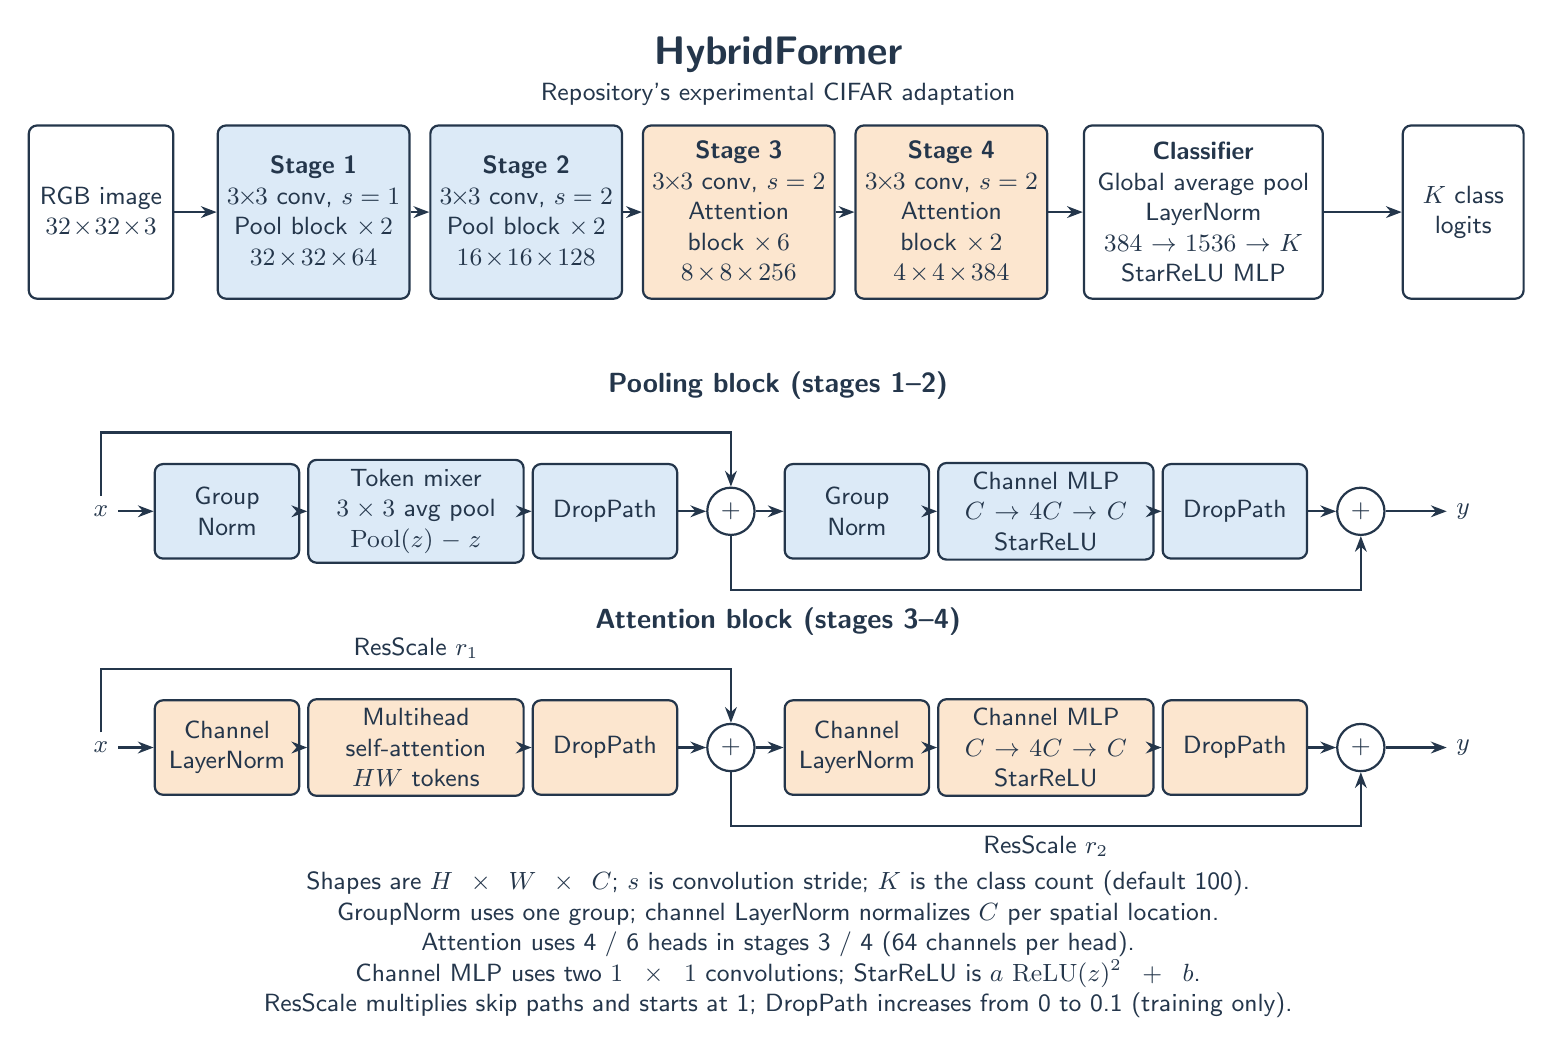
\begin{tikzpicture}[font=\sffamily\small,text=ink]
  \node[font=\sffamily\bfseries\Large] at (8.6,2) {HybridFormer};
  \node at (8.6,1.5) {Repository's experimental CIFAR adaptation};
  \node[box,fill=white,text width=16mm] (input) at (0,0)
    {RGB image\\$32\!\times\!32\!\times\!3$};
  \node[box] (s1) at (2.7,0)
    {\textbf{Stage 1}\\$3\!\times\!3$ conv, $s=1$\\Pool block $\times\,2$\\$32\!\times\!32\!\times\!64$};
  \node[box] (s2) at (5.4,0)
    {\textbf{Stage 2}\\$3\!\times\!3$ conv, $s=2$\\Pool block $\times\,2$\\$16\!\times\!16\!\times\!128$};
  \node[box,fill=attentionorange] (s3) at (8.1,0)
    {\textbf{Stage 3}\\$3\!\times\!3$ conv, $s=2$\\Attention block $\times\,6$\\$8\!\times\!8\!\times\!256$};
  \node[box,fill=attentionorange] (s4) at (10.8,0)
    {\textbf{Stage 4}\\$3\!\times\!3$ conv, $s=2$\\Attention block $\times\,2$\\$4\!\times\!4\!\times\!384$};
  \node[box,fill=white,text width=28mm] (head) at (14,0)
    {\textbf{Classifier}\\Global average pool\\LayerNorm\\$384\to1536\to K$\\StarReLU MLP};
  \node[box,fill=white,text width=13mm] (output) at (17.3,0) {$K$ class\\logits};
  \draw[flow] (input) -- (s1);
  \draw[flow] (s1) -- (s2);
  \draw[flow] (s2) -- (s3);
  \draw[flow] (s3) -- (s4);
  \draw[flow] (s4) -- (head);
  \draw[flow] (head) -- (output);

  \node[font=\sffamily\bfseries] at (8.6,-2.2) {Pooling block (stages 1--2)};
  \node (px) at (0,-3.8) {$x$};
  \node[op] (pn1) at (1.6,-3.8) {Group\\Norm};
  \node[op,text width=25mm] (pmix) at (4,-3.8)
    {Token mixer\\$3\times3$ avg pool\\$\operatorname{Pool}(z)-z$};
  \node[op] (pd1) at (6.4,-3.8) {DropPath};
  \node[sum] (pa1) at (8,-3.8) {$+$};
  \node[op] (pn2) at (9.6,-3.8) {Group\\Norm};
  \node[op,text width=25mm] (pmlp) at (12,-3.8)
    {Channel MLP\\$C\to4C\to C$\\StarReLU};
  \node[op] (pd2) at (14.4,-3.8) {DropPath};
  \node[sum] (pa2) at (16,-3.8) {$+$};
  \node (py) at (17.3,-3.8) {$y$};
  \draw[flow] (px) -- (pn1);
  \draw[flow] (pn1) -- (pmix);
  \draw[flow] (pmix) -- (pd1);
  \draw[flow] (pd1) -- (pa1);
  \draw[flow] (pa1) -- (pn2);
  \draw[flow] (pn2) -- (pmlp);
  \draw[flow] (pmlp) -- (pd2);
  \draw[flow] (pd2) -- (pa2);
  \draw[flow] (pa2) -- (py);
  \draw[flow] (px.north) -- (0,-2.8) -- (8,-2.8) -- (pa1.north);
  \draw[flow] (pa1.south) -- (8,-4.8) -- (16,-4.8) -- (pa2.south);

  \node[font=\sffamily\bfseries] at (8.6,-5.2) {Attention block (stages 3--4)};
  \node (ax) at (0,-6.8) {$x$};
  \node[op,fill=attentionorange] (an1) at (1.6,-6.8) {Channel\\LayerNorm};
  \node[op,fill=attentionorange,text width=25mm] (amix) at (4,-6.8)
    {Multihead\\self-attention\\$HW$ tokens};
  \node[op,fill=attentionorange] (ad1) at (6.4,-6.8) {DropPath};
  \node[sum] (aa1) at (8,-6.8) {$+$};
  \node[op,fill=attentionorange] (an2) at (9.6,-6.8) {Channel\\LayerNorm};
  \node[op,fill=attentionorange,text width=25mm] (amlp) at (12,-6.8)
    {Channel MLP\\$C\to4C\to C$\\StarReLU};
  \node[op,fill=attentionorange] (ad2) at (14.4,-6.8) {DropPath};
  \node[sum] (aa2) at (16,-6.8) {$+$};
  \node (ay) at (17.3,-6.8) {$y$};
  \draw[flow] (ax) -- (an1);
  \draw[flow] (an1) -- (amix);
  \draw[flow] (amix) -- (ad1);
  \draw[flow] (ad1) -- (aa1);
  \draw[flow] (aa1) -- (an2);
  \draw[flow] (an2) -- (amlp);
  \draw[flow] (amlp) -- (ad2);
  \draw[flow] (ad2) -- (aa2);
  \draw[flow] (aa2) -- (ay);
  \draw[flow] (ax.north) -- (0,-5.8) -- node[above] {ResScale $r_1$} (8,-5.8) -- (aa1.north);
  \draw[flow] (aa1.south) -- (8,-7.8) -- node[below] {ResScale $r_2$} (16,-7.8) -- (aa2.south);

  \node[align=center,text width=175mm] at (8.6,-9.3)
    {Shapes are $H\times W\times C$; $s$ is convolution stride; $K$ is the class count (default 100).\\
     GroupNorm uses one group; channel LayerNorm normalizes $C$ per spatial location.\\
     Attention uses 4 / 6 heads in stages 3 / 4 (64 channels per head).\\
     Channel MLP uses two $1\times1$ convolutions; StarReLU is $a\,\operatorname{ReLU}(z)^2+b$.\\
     ResScale multiplies skip paths and starts at 1; DropPath increases from 0 to 0.1 (training only).};
\end{tikzpicture}
\end{document}
